\documentclass{article}
\usepackage{graphicx}
\usepackage{amsmath}

\title{Assessment of Pitch Estimation Algorithm for Single-note Instrument Sound Recordings}
\author{Akke Houben}
\date{2016}

%\begin{figure}
%	\includegraphics{img/plan_tot.jpg}
%	\caption{Total plan of the system}
%	\label{fig:total}
%\end{figure}

\begin{document}
\maketitle

% --------------------------------------------------------------------------------------|
% Introduction
% --------------------------------------------------------------------------------------|
\section{Introduction}
Freesound\footnote{http://freesound.org/} is a project initiated and maintained by the Music Technology Group of the Universitat Pompeu Fabra (Barcelona) \footnote{http://mtg.upf.edu/} with the aim to "create a huge collaborative database of audio snippets, samples, recordings, bleeps, ... released under Creative Commons licenses that allow their reuse." and "to create an open database of sounds that can also be used for scientific rescearch and be integrated in third party applications." (http://freesound.org/). Following these aims efforts are undertaken to present the collection of sounds is multiple ways. This database contains a vast collection of single-note instrument sounds, which can be perfectly usable to use in software sample synthesisers to create digital instruments which are playable with for instance a MIDI keyboard. However it is a challenge to automatically collect the right sounds together and to make sure all the needed sounds are found or created. This current article will adres the problem of pitch estimation of single-note sounds. It is important to be able to get reliable pitch estimates as the software sample synthesiser demands that the rightly pitched sound is placed under the right keyboardkey. The Freesound pitch estimation is done using the pitchYinFFT algorithm contained in the Essentia library (Bogdanov, et al., 2013; http://essentia.upf.edu/). The pitchYinFFT is a optimalisation proposed by Brossier (Brossier, 2007) for reduced calculation time of the YIN algorithm of Cheveigné and Kawahara (Cheveigné & Kawahara, 2002; Bogdanov, et al., 2013). 
In this document the performance of the pitch estimation algorithm used by Freesound to estimate the pitches of sounds on single-note sounds will be assessed. The method used in this assessment is quite straight forward. A large collection of annotated sounds is gathered from Freesound and two other sources\footnote{Attached is a desription of the sounds used in this assessment as well as a comparison between the pitch estimates taken from Freesound and the locally computed estimates.}.
 This assessment will consist of a observation of the quality of the estimation (1), followed by a discussion on factors able to predict the quality of this estimation (2). Lastly possible improvements to the algorithm or the useage of the algorithm will be proposed and discussed (3).
% --------------------------------------------------------------------------------------|

% --------------------------------------------------------------------------------------|
% Performance of pitch estimation
% --------------------------------------------------------------------------------------|
\section{Performance of the pitch estimation}
\subsection{Method}
The performance of the pitch estimation algortihm will be assessed by comparing the pitch estimated by the algorithm against the pitch annotated for that sound, taken either from the filename or the descriptions and/or tags of the sounds. In this section the usage of the pitchYinFFT is the same as is implemented in Freesound. 
% /Method

\subsection{Results}
% /Results
Figure \ref{fig:pTag_distr} shows the distribution of the annotated pitches and figure \ref{fig:pEst_distr} shows the distribution of corresponding estimated pitches. The mean difference between the annotated and estimated pitches is $109Hz$ ($\sigma = 504.5Hz$). Around $58\%$ of the sounds are estimated higher than they are annotated. In table \ref{table:pTag_pEst} some statistical values of the annotated and estimated pitches are given.

\begin{figure}
    \centering
    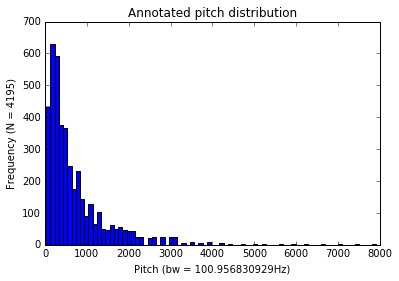
\includegraphics[scale=0.5]{pTag_distribution.png}
    \caption{Distribution of annotated pitches}
    \label{fig:pTag_distr}
\end{figure}
\begin{figure}
    \centering
    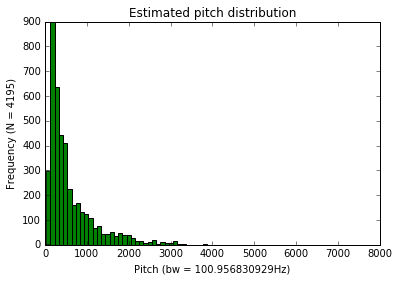
\includegraphics[scale=0.5]{pEst_distribution.png}
    \caption{Distribution of estimated pitches}
    \label{fig:pEst_distr}
\end{figure}
\begin{figure}
    \centering
    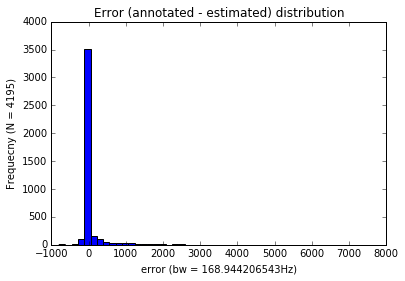
\includegraphics[scale=0.5]{err_distribution.png}
    \caption{Distribution of errors (annotation - estimation)}
    \label{fig:err_distr}
\end{figure}

\begin{table}[h]
    \begin{center}
        \begin{tabular}{ | l | c | c | r |}
            \hline
                        &   mean:       &   std:        &   median:     \\  \hline
            Annotated:  &   $711.7Hz$   &   $749.0Hz$   &   $440.0Hz$   \\  \hline
            Estimated:  &   $602.4Hz$   &   $584.2Hz$   &   $390.2Hz$   \\  
            \hline
        \end{tabular}
        \caption{Annotated and Estimated pitches}
        \label{table:pTag_pEst}
    \end{center}
\end{table}
As pitch is clearly a human percept it is more usefull not to talk in terms of frequencies, but some other scale. Below the error values are converted to Equivalent Rectangular Bandwidths and to semitones. In the rest of this document the semitone difference is used, as this is a in the scope of the current project an understandable and meaningfull measure. 

\begin{figure}
    \centering
    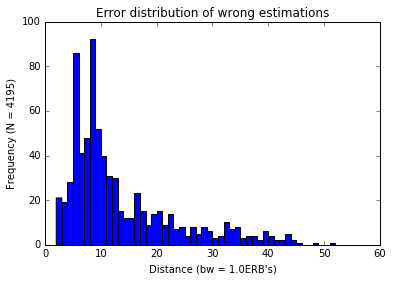
\includegraphics[scale=0.5]{erb_distribution.png}
    \caption{Distribution of ERB distances of wrong estimates}
    \label{fig:erb_distr}
\end{figure}

\begin{figure}
    \centering
    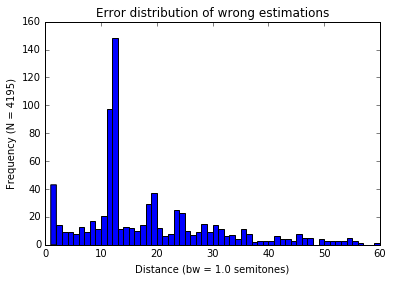
\includegraphics[scale=0.5]{st_distribution.png}
    \caption{Distribution of semitone distances of wrong estimates}
    \label{fig:st_distr}
\end{figure}

\begin{table}[h]
    \begin{center}
        \begin{tabular}{ | l | c | c | c || r |}
            \hline
                        &   mean:       &   std:        &   median:     &   $distance < 1$:\\  \hline
            ERBs:       &   $3.12ERBs$  &   $6.15ERBs$  &   $1.00ERBs$  &   $82.34\%$   \\  \hline
            semitones:  &   $3.58st$    &   $8.95st$    &   $0.12st$    &   $81.33\%$   \\  
            \hline
        \end{tabular}
        \caption{ERB and semiton distances}
        \label{table:ERB_st}
    \end{center}
\end{table}

From this point onward the estimations with a difference between the estimation and annotation of less than one semitone are called 'correct estimations'. Estimations with a difference bigger or equal to one semitone are called 'incorrect estimations'.

Figure \ref{fig:erb_distr} shows that around $82\%$ of the estimations fall within the same ERB as the annotated pitch and figure \ref{fig:st_distr} shows that $81\%$ of the estimations differ less than 1 semitone from the annotated pitch.

A common error in pitch estimations are ocatve errors (Gerhard, 2003), here the pitch is estimated to be a (sub) harmonic of the annotated pitch of the sound. Figure \ref{fig:st_distr} shows a clear peak in the bands corresponding to a distance of 12 semitones. Around $52.36\%$ of the errors can be identified as octave errors using the histogram of figure \ref{fig:octerr1}.

\begin{figure}
    \centering
    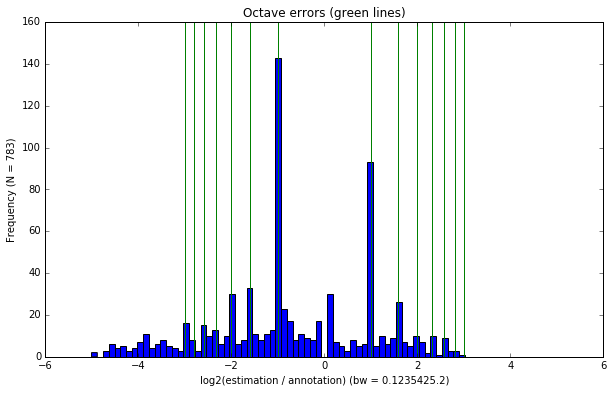
\includegraphics[scale=0.5]{octerr1.png}
    \caption{Octave Errors}
    \label{fig:octerr1}
\end{figure}

\subsection{Discussion}
As can be seen from figure \ref{fig:err_distr} most errors fall within a bandwidth close to 0Hz. However the mean of the point-wise errors is around 109Hz. Looking at the mean error and the mean and median values of the annotated versus the estimated pitches the pitch estimator tends to estimate pitches lower than the anntotation. However when the median value of the point-wise errors and the percentage of sounds with a higher annotation than estimation, suggest that there are some big differences where the estimation is cosiderably lower than the annotation. Also the median of the point-wise errors lies very close to 0Hz thus it can be inferred that no clear tendency to estimate too low or too high can be determined.

Figure \ref{fig:st_distr} and figure \ref{fig:octerr1} show that quite a lot of errors can be identified as octave errors. A clear improvement can be made by reducing the chance of octave errors occurring.
% --------------------------------------------------------------------------------------|

% --------------------------------------------------------------------------------------|
% Prediction of Errors
% --------------------------------------------------------------------------------------|
\section{Prediction of Errors}
In this section measurements to predict the performance of the estimation are investigated. Firstly predictors for the amplitude of the errors are looked at. After this factors which indicate the occurence of octave errors will be investigated.

\subsection{Method}
Several measurements will be investigated for their usefullness as predictors for the correctness of the estimates. Firstly some values returned by the pitchYinFFT and one measure directly related to the tonality of the signal are discussed. Secondly some other tonal and aural descriptors which can predict high error values are searched. The methods used to determine the usefullness of each measurement are fourfold:
\begin{enumerate}
    \item Firstly the difference in the mean of the values of the measurements between the correctly and incorrectly estimated sounds, the bigger this difference the more usefull the measurement. 
    \item Secondly the descriptors are tested for their abilities to correctly identify what sounds will be correctly estimated. The descriptors which acceptations and rejections coincide mostly with respectively the correctly and the incorrectly estimated sounds (highest percetage of true positives and true negatives) are most potent as predictors. 
    \item Thirdly a line is fitted trough the datapoints (predictor value, semitone distance), afterwards the distance between the fitted line and each datapoint is taken as an prediction error measurement. A low prediction error means a better predictor quality.
    \item Lastly the 'Select Attributes' functionality from Weka (http://www.cs.waikato.ac.nz/ml/weka/) using as Attribute Evaluator the 'InfoGainAttributeEval' and as Search Method the 'Ranker' is used.
\end{enumerate}
When considering predictors for octave errors, octave errors are considered 'incorrect estimations' and all estimates which are no octave errors are considered 'correct estimations'
\subsection{Results}


\subsection{Discussion}
%Due to the characteristics of the algorithms used in the pitchYinFFT pitch estimation some type of sounds could be 


% --------------------------------------------------------------------------------------|

% --------------------------------------------------------------------------------------|
% Improvements
% --------------------------------------------------------------------------------------|
\section{Improvements}

\subsection{Method}

\subsection{Results}

\subsection{Discussion}


% --------------------------------------------------------------------------------------|

% --------------------------------------------------------------------------------------|
% Conclusion
% --------------------------------------------------------------------------------------|
\section{Conclusion}
% --------------------------------------------------------------------------------------|

% --------------------------------------------------------------------------------------|
% References
% --------------------------------------------------------------------------------------|


\section{References}

\end{document}
